
\documentclass[a4paper, 12pt]{article}

\usepackage[french]{babel} 
\usepackage[utf8]{inputenc}
\usepackage[T1]{fontenc} 
\usepackage{amsmath}
\usepackage[toc,page]{appendix}
\usepackage{amssymb}
\usepackage{listings}  
\usepackage{graphicx}
\usepackage[margin=2.5cm]{geometry}
\usepackage{amsmath,amsfonts,amssymb}
\usepackage{hyperref}
\lstset{
language=Java,
breaklines=true
}



\newcommand*{\plogo}{\fbox{$\mathcal{PL}$}} % Generic publisher logo

%----------------------------------------------------------------------------------------
%	TITLE PAGE
%----------------------------------------------------------------------------------------

\newcommand*{\titleGM}{\begingroup % Create the command for including the title page in the document
\hbox{ % Horizontal box
\hspace*{0.2\textwidth} % Whitespace to the left of the title page
\rule{2pt}{\textheight} % Vertical line
\hspace*{0.05\textwidth} % Whitespace between the vertical line and title page text
\parbox[b]{0.75\textwidth}{ % Paragraph box which restricts text to less than the width of the page

{\noindent\Huge\bfseries Software Project\\ Engineering }\\[2\baselineskip] % Title
{\Large \textit{Phase 4 Report}}\\[4\baselineskip] % Tagline or further description
{\Large \textbf{Project leader} : Hélène Verhaeghe}
\\
{\Large \textsc{\textbf{Group E}}\\\textsc{Aurian De Potter(Group leader)},\\ \textsc{Eddy Ndizera},\\ \textsc{Ivan Ahad},\\ \textsc{Arnaud Dethise},\\ \textsc{Ludovic Fastré},\\ \textsc{Anthony Dechamps},\\ \textsc{Geoffroy Husson},\\ \textsc{Jonathan Legat}} % Author name

\vspace{0.5\textheight} % Whitespace between the title block and the publisher
{\noindent \Large \textbf{INGI2255}}\\[\baselineskip] % Publisher and logo
}\\

}
\endgroup}


\clearpage
\setcounter{page}{0}
\begin{document}
\titleGM
\section{Introduction}
We will start the \textit{Phase 4} report by a summary of our meeting with the client. We will then explain how the implementation of the requirements planned for this phase is going, and give information about the evolution of the architecture of our program. For this phase, we had to submit our code to the project. It is available in section 3.3, by following our GitHub repository.

\section{Meeting with client}

Last week, we had an appointment with the client, we will briefly explain here what was his feedback of the live version of our website. \\

We started off the meeting by asking a few questions that will allow us to improve the software.\\

We were wondering if it was important to keep tracks of the logins. The client responded that it was an important feature and should be generalized to track all actions done by staff members (update of players informations, etc). This will be implemented during the final phase.\\

We also asked if it was important to display the prices of registration, which it indeed was as a player would like to know how much he need to pay without having to count by himself.//

It was also necessary to have a smart registration, where the members of a pair fill their information and they're immediately assigned to a tournament. However, if a user doesn't match any tournament, there must be a message that clearly shows that getting a match wasn't possible. We can also display a message to show which tournament a pair has been assigned to. This feature was added partially. We assign automatically a pair or solo player to a tournament based on their gender and age. But we don't advertise them about which tournament they've been assigned.\\

Lastly, as a court is assigned to a pool, we were told that the courts must be assigned according to how close it is to the headquarters. As thus, the staff members should be able to manually be able to set a court to a pool. The client said that we could implement an algorithm to do so, but it was not  an important feature.\\

We also received some feedback on other functionalities. He said it was a good idea to have a \textit{wiki}, since the organisation already uses one,for other websites and the home page was good. We could add some explanation about the tournaments but we must keep in mind that people usually come to the website only for registration and not to read the informations on the website.\\ 

The \textit{Court tab} isn't very clear, and in the Tournament tab, we must not show publicly where people play in advance, because they must first come to the headquarters to pay for their registration. We will add a tournament tab for the final phase in the visitor pages (which has been removed) so as to give a pdf file of the pools but will be accessible only the day of the tournament.\\

Some more feedbacks : it is better to not display the final score of a match because some players don't like others to see their scores when they lose (like 6-0), putting the type of courts  as a list which can be terre battue, béton, ... when registering a court. A staff member must be able to manually edit a pool (when a tournament is created, a staff member can manually modify the pairs in a pool). More generally, we must make everything manually changeable.
The two last features has been implemented. For the first one, as we don't let visitors see the scores of the tournament, this feedback is respected.
\newpage
\section{Requirements, software description, Changes according to feedback}

The requirements below are the ones we planned to develop for the second phase. This time, every requirement has been implemented. \\
\subsection{For this phase}
	
\begin{itemize}
 
\item Files sharing between staff members (Eddy, Aurian)
\item Communication channel between staff members (Eddy)
\item The user can use a payment method among several options (Aurian)
\item The system must query AFT rankings (Optional)(See below)
\item The system can create smaller pools when it rains (Optional)(See below)
\\
\end{itemize}

It is important to note that the requirements haven't been implemented in this particular order.\\

You can see in the list above who implemented which requirement(s) for this phase. 

\subsection{Implementation \& choices}

Here are a few other features that we implemented during this phase. \\

Upon encoding all the scores of the matches in a pool, the winner of this group is displayed in green and the knock-off tournament is created in the database. Plus, it is now possible to see the bracket with a pretty graphical version. The players that are the winners of a group will then get to the bracket. The scores are, for now, only editable by an admin account. Another feature that was added is that a user can now delete his own email address from the database, so that he can delete his own information on his own.\\

For the implementation of \textit{"The system must query AFT rankings" and "The system can create smaller pools when it rains"}, as these two functionalities were optional, we decided not to implement them. It thought it would take too much time to do so, and that implementing wouldn't be a great benefit after all.\\

As you can see, there weren't many requirements as scheduled for this phase. As stated in the previous report, this phase was much more dedicated to improving some underlying functionalities of the website to make it easier to use.

\subsubsection*{Implementations according to meeting with client}

First of all, as requested, we implemented a system that allows to exchange messages. We also added a system that allows to share files that they can upload/download. The staff members already have other means to communicate, so these two features are important for very important announcements. They are available on a dedicated page. You can see in figure \ref{annonce} below how a staff member can put an announcement, and how one can upload files in figure \ref{file} \\
\begin{figure}[h]
  \caption{\label{annonce} Announcement creation}
  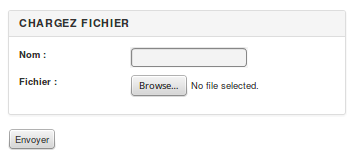
\includegraphics[scale=0.7]{annonce.png}
\end{figure}
\begin{figure}[h]
  \caption{\label{file} File sharing}
  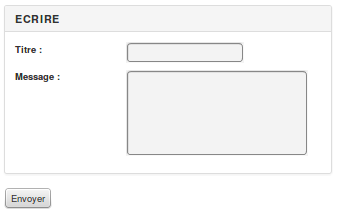
\includegraphics[scale=0.7]{fichier.png}
\end{figure}


It is also now possible to modify the pools by taking into account the commentaries made.\\

We also added a functionality that allows to look for players and courts, but also pairs. We then added a list of all the players and all the courts.

\subsubsection*{Changes during registration}
Secondly, we focused on modifying the registration of a player, as it was asked by the client. We have implemented the smart registration, where a player is automatically assigned to a tournament according to his information.\\

Moreover, when a form is filled, there is a summary of all the player information, allowing him to check what he is going to pay afterwards. You can see in figure \ref{recap} how the information is presented after validation.

\begin{figure}[h]
  \caption{\label{recap} Summary of player information}
  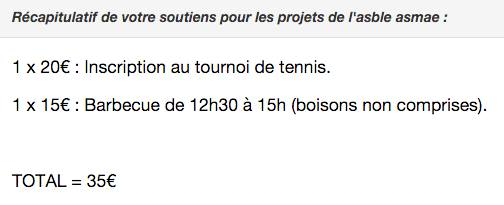
\includegraphics[scale=0.7]{recap.png}
\end{figure}

Another modification is that now the payment choice is chosen after a user has entered and validated all his information.
\subsubsection*{Bugs fixed}
In the last sprint, it was said in the previous report that the staff member interface had a different background to differenciate the navigation between a simple user and a staff user. We actually submitted a wrong live version where this feature was not implemented yet, which is now fixed.\\

One bigger issue was that we implemented a functionality that allowed to use an email so that a user doesn't have to fill all his information. By using the email, the system retrieved all the information from a past registration. However, this feature lead to information leak. From that point, we had to make a decision : we decided to send a confirmation email with a link, this link sends a token that allows the user to be recognized and to display his information. It is important to notice that in the case of a pair, only the information of the one who entered his email will be displayed, the other one will have to manually fill his form. It is a choice to have a more secured system, especially when two players are joined as a pair and if they're unknown to each other. We decided to implement this functionality in the last phase.\\

Some other bugs such as getting an error when trying to modify a user while being logged as a staff member, or one player couldn’t register alone leading to an error, or when logged as staff member when clicking on a tournament it changed to a user tournament. Those problems have all been fixed as well.

\subsection{The software}


Here is the live version of our website : http://sep2015e.herokuapp.com.  To get admin access you should add "/admin" in the url.\\

\textbf{To get access to the code of our project}, you can click on the link to our \textit{Github} repository : https://github.com/ivanahad/sep2015E\\
\subsubsection*{How to modify a tournament}

\section{For next phase}
\subsection{Tests to improve the software}
To improve our software, we are going to ask random people to test the website to see if it is user-friendly and easy to use, and then we will proceed to modify it accordingly.\\

We will also navigate randomly to search for bugs and strange behaviors that may arise after modifications of the database.\\
 
We will also test our website on different monitors with different screen sizes to see if it fits the window correctly.\\

\subsection{Documentation}
The documentation will be one of our main focuses. It will be divided into two parts: the first will be dedicated for the staff and admin and the second for the maintainer of the website. For the admin and staffs, the documentation will be a guide on how to navigate on the website and on how to basic stuffs like as modifying a pool, editing a player, etc. This documentation will be found on a wiki but links will be on the website to directly access the content specific to a part of the website. For the maintainer of the code, the documentation will be more technical. We will explain our implementaion, what we use and how we do it. 



\newpage
\section{Architecture discussion, choices \& UML Diagram}

You can see our UML diagram in Figure\ref{uml}. Since the last phase, we changed.\\

In the architecture, in this phase, there isn't much that has changed. However, one big change is that we added many methods that now allow to modify information about users, courts, tournaments, etc. Making things changeable manually was one of our main coucerns for this phase, as it was requested by the client.

\begin{figure}[b]
	\centering
 	\caption{\label{uml} UML diagram}
	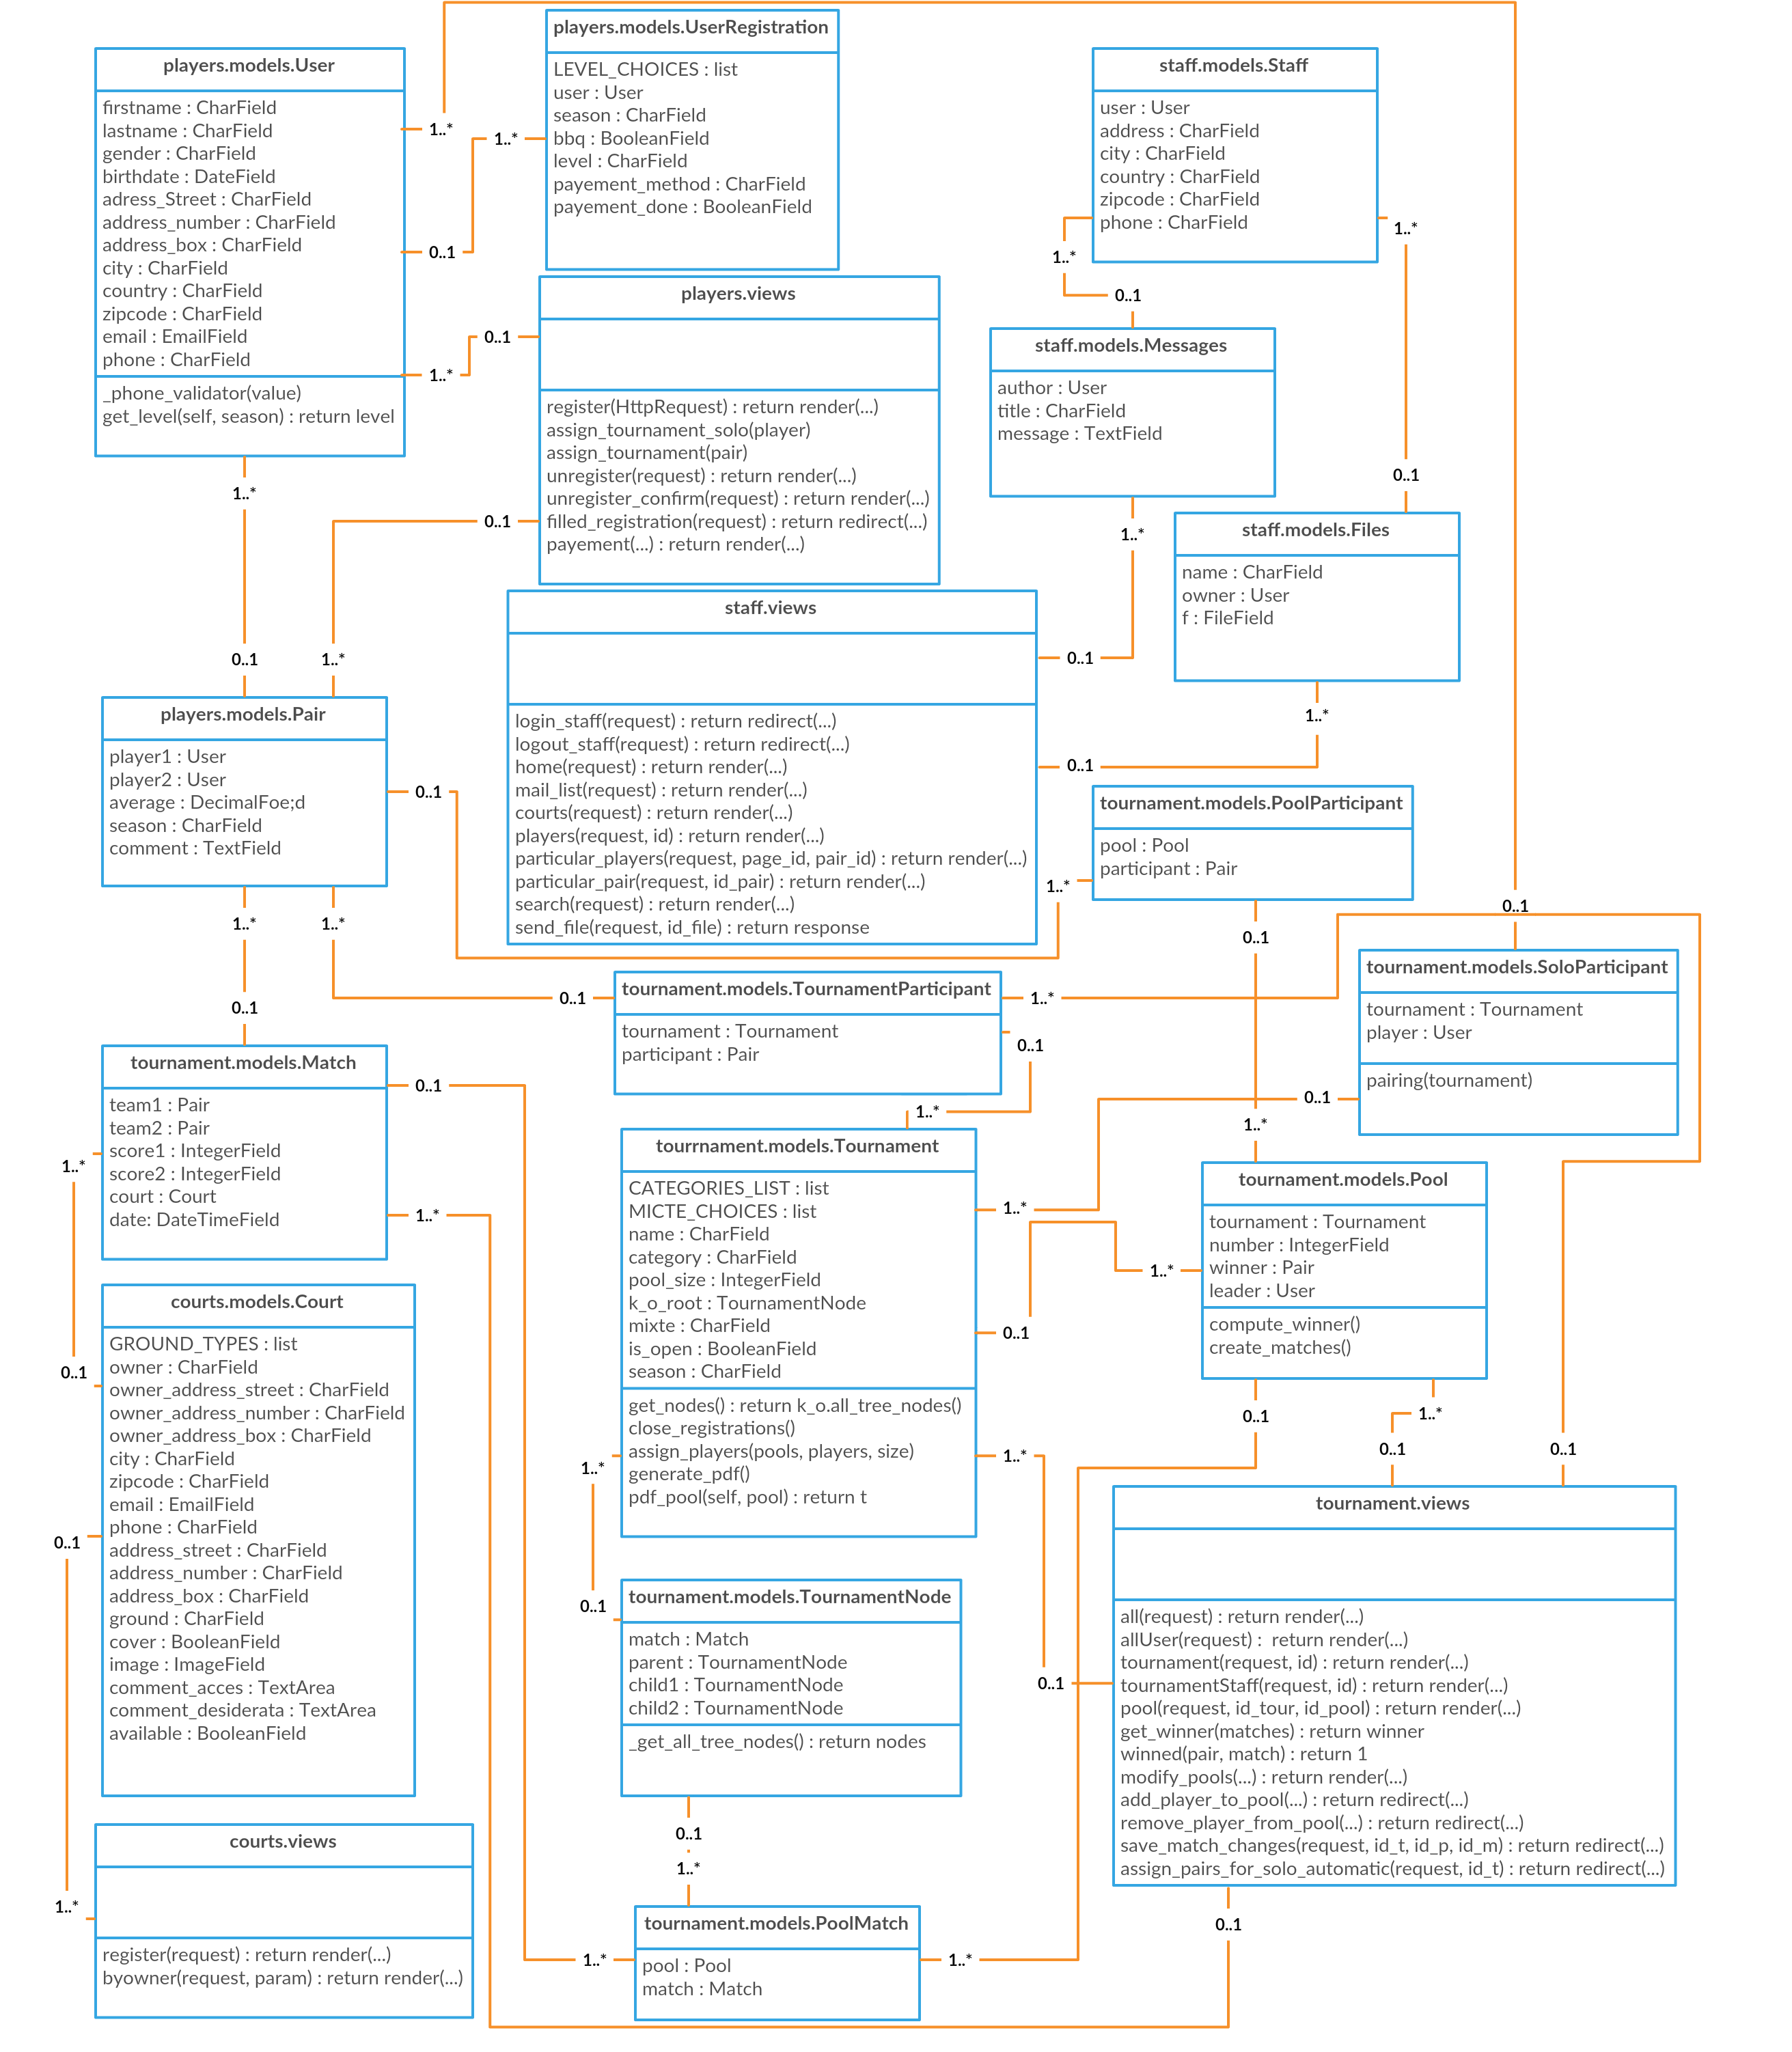
\includegraphics[scale=0.2]{Class.png}
\end{figure}

\subsection*{Sequences diagram}

You can see in figure \ref{sequence} the sequence diagram for how a player registers to a tournament with an email confirmation. It has been updated since the last phase's report.

\begin{figure}[position]
   \caption{\label{playerseq} Sequence diagram}
  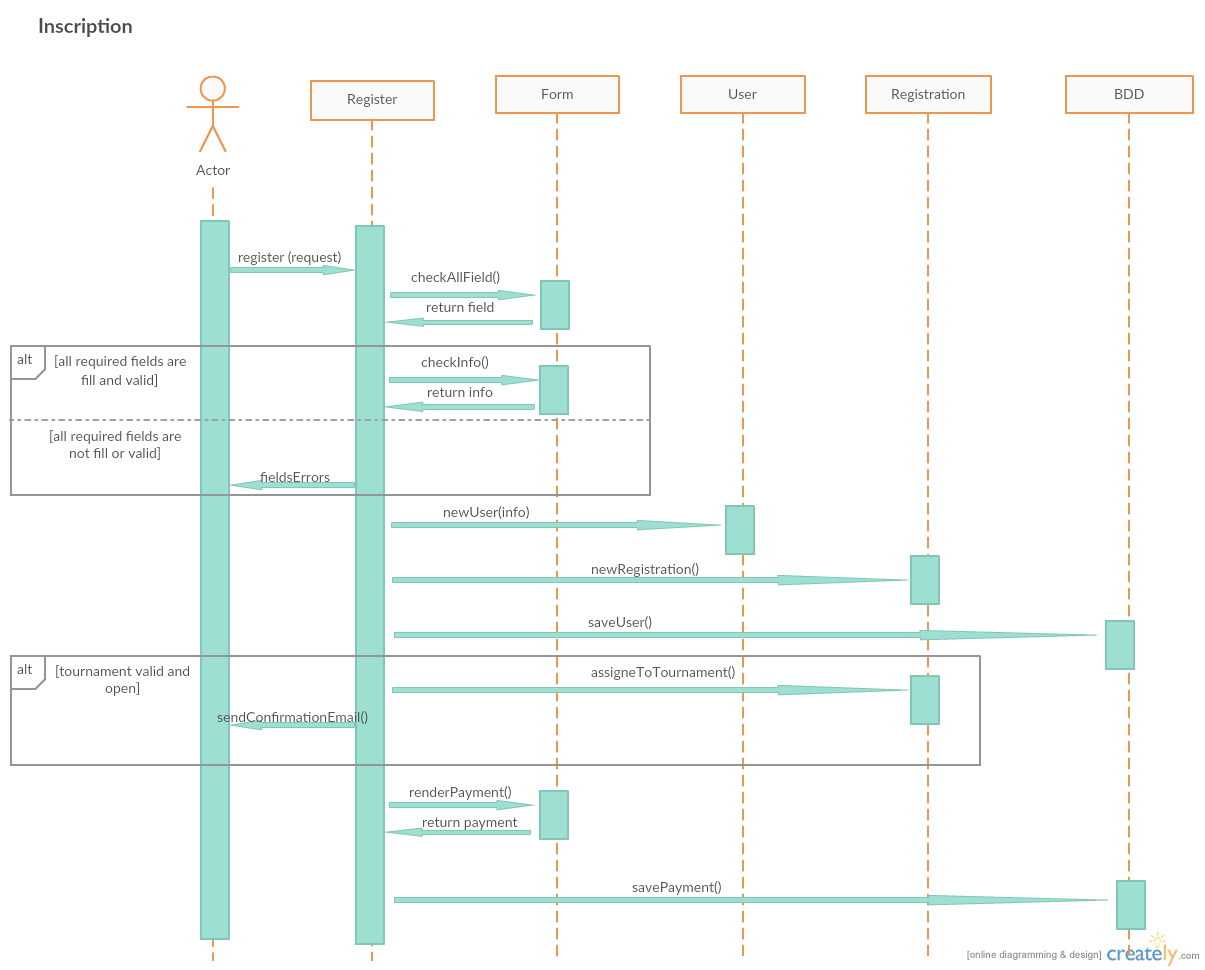
\includegraphics[scale=0.4]{Inscription.png}
\end{figure}
The second sequence diagram describes the life cycle of a tournament, how players are added into groups, how the knock-off tournament is created, how the tournament is created, etc. 

\begin{figure}[position]
   \caption{\label{tournseq} Sequence diagram for tournament}
  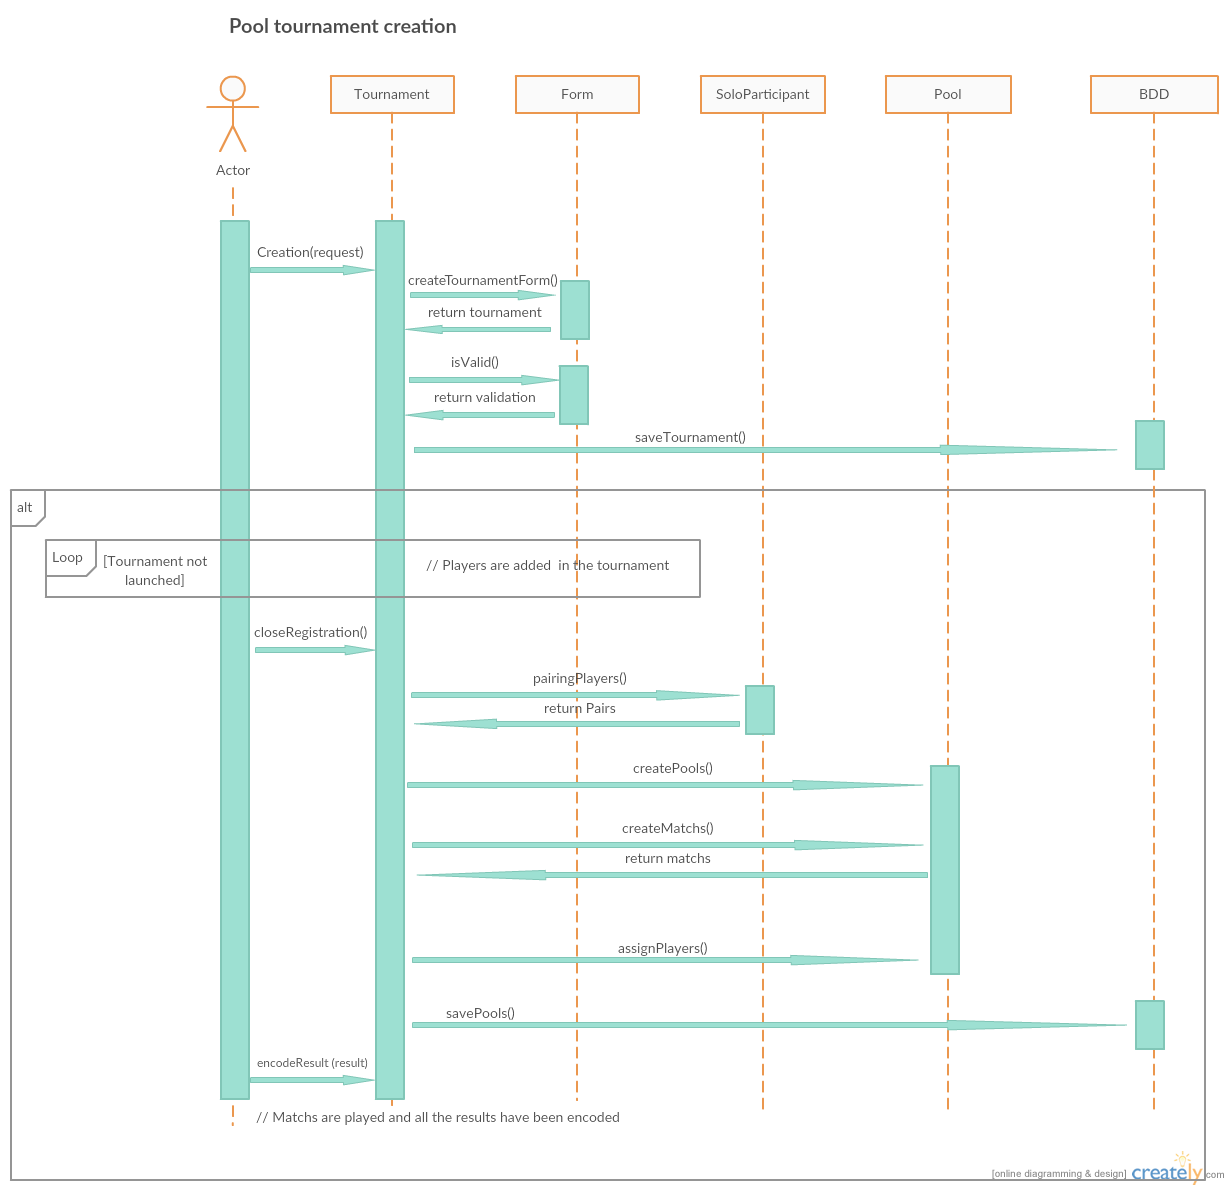
\includegraphics[scale=0.4]{Tournament.png}
\end{figure}


\section{Conclusion}

For this phase, we modified our software according to our meeting. We mainly focused on correcting bugs and making the website more user-friendly.

\end{document}